\section{The Region Connection Calculus family (RCC)}

The calculi from the RCC family (RCC-8 and RCC-5) allow
mereotopological reasoning (reasoning about connection and
part-of relationships) about simple regions in
the plane. Other domains involving regions
can also be considered in the context of RCC, e.g.\
3D regions, or non-simple regions in the plane,
which can affect the correctness of the
constraint-based reasoning algorithms.
Since so far no qualifier for RCC is available in \engine{},
the exact domain is actually still not determined. However, we
will assume the case of simple regions in the plane
in the following.


\subsection*{RCC-8}\label{sec:rcc8}

\kasten{
\subsubsection*{Region Connection Calculus 8 (RCC-8) overview}
\begin{calcfeatures}
\feature{calculus identifier}{rcc-8}
\feature{calculus parameters}{none}
\feature{arity}{binary}
\feature{entity type}{simple regions in the plane}
\feature{description}{describes the mereotopological relation between two regions}
\feature{base relations}{dc (disconnected), ec (externally connected),
po (partially overlapping), eq (equal), tpp (tangential proper part), ntpp (non-tangential proper part), tppi (tangential proper part inverse), ntppi (non-tangential proper part inverse)}
\feature{references}{\citet{randell92_rccb,Cohn97a}}
\lastfeature{remarks}{no qualifier is available for this calculus yet}
\end{calcfeatures}
}

RCC-8 is the more fine-grained variant of RCC calculi. It distinguishes
the eight base relations  dc (disconnected), ec (externally connected),
po (partially overlapping), eq (equal), tpp (tangential proper part), ntpp (non-tangential proper part), tppi (tangential proper part inverse), and nttpi (non-tangential proper part inverse) which are illustrated in Fig.~\ref{fig:RCC8}.

\begin{figure}[ht]
	\centering
	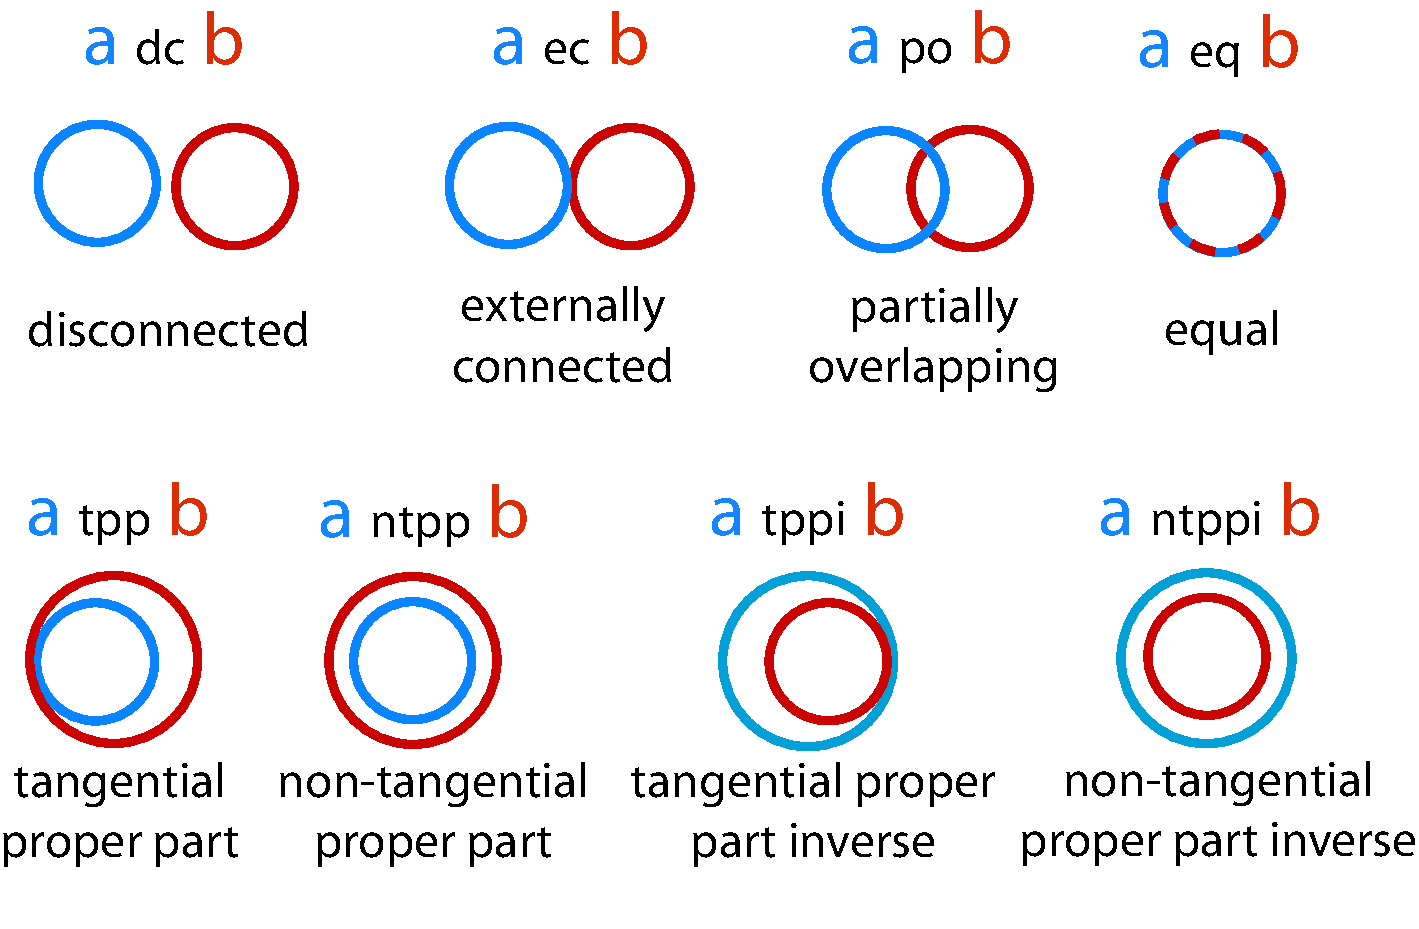
\includegraphics[width=0.70\textwidth]{RCC_new2}
	\caption{The RCC-8 base relations.}
	\label{fig:RCC8}
\end{figure}

\subsection*{RCC-5}\label{sec:rcc5}

\kasten{
\subsubsection*{Region Connection Calculus 5 (RCC-5) overview}
\begin{calcfeatures}
\feature{calculus identifier}{rcc-5}
\feature{calculus parameters}{none}
\feature{arity}{binary}
\feature{entity type}{simple regions in the plane}
\feature{description}{describes the mereotopological relation between two regions}
\feature{base relations}{dr (discrete from), po (partially overlapping), eq (equal),
pp (proper part), ppi (proper part inverse)}
\feature{references}{\citet{Cohn97a}}
\lastfeature{remarks}{no qualifier is available for this calculus yet}
\end{calcfeatures}
}

RCC-5 is a coarser version of RCC-8.  The RCC-8 relations
dc and ec are combined into one relation called dr. Similarly,
ntpp and tpp are combined into pp and ntppi and tppi into ppi.


